\documentclass[aspectratio=169]{beamer}
\mode<presentation>
\usetheme{Hannover}
\useoutertheme{sidebar}
\usecolortheme{dolphin}

\usepackage{amsmath}
\usepackage{amssymb}
\usepackage{enumerate}


% some bold math symbosl
\newcommand{\Cov}{\mathrm{Cov}}
\newcommand{\Cor}{\mathrm{Cor}}
\newcommand{\Var}{\mathrm{Var}}
\newcommand{\brho}{\boldsymbol{\rho}}
\newcommand{\bSigma}{\boldsymbol{\Sigma}}
\newcommand{\btheta}{\boldsymbol{\theta}}
\newcommand{\bbeta}{\boldsymbol{\beta}}
\newcommand{\bmu}{\boldsymbol{\mu}}
\newcommand{\bW}{\mathbf{W}}
\newcommand{\one}{\mathbf{1}}
\newcommand{\bH}{\mathbf{H}}
\newcommand{\by}{\mathbf{y}}
\newcommand{\bolde}{\mathbf{e}}
\newcommand{\bx}{\mathbf{x}}

\newcommand{\cpp}[1]{\texttt{#1}}

\title{Mathematical Biostatistics Bootcamp: Lecture 10, T Confidence Intervals}
\author{Brian Caffo}
\date{\today}
\institute[Department of Biostatistics]{
  Department of Biostatistics \\
  Johns Hopkins Bloomberg School of Public Health\\
  Johns Hopkins University
}


\begin{document}

\frame{\titlepage}


\section{Table of contents}
\frame{
  \frametitle{Table of contents}
  \tableofcontents
}

\section{Independent group $t$ intervals}
\begin{frame}\frametitle{Independent group $t$ confidence intervals}
  \begin{itemize}
  \item Suppose that we want to compare the mean blood pressure between
    two groups in a randomized trial; those who received the treatment
    to those who received a placebo
  \item We cannot use the paired t test because the groups are independent
    and may have different sample sizes
  \item We now present methods for comparing independent groups
  \end{itemize}
\end{frame}

\begin{frame}\frametitle{Notation}
  \begin{itemize}
  \item Let $X_1,\ldots,X_{n_x}$ be iid $N(\mu_x,\sigma^2)$
  \item Let $Y_1,\ldots,Y_{n_y}$ be iid $N(\mu_y, \sigma^2)$
  \item Let $\bar X$, $\bar Y$, $S_x$, $S_y$ be the means and standard deviations
  \item Using the fact that linear combinations of normals are again normal, we
    know that $\bar Y - \bar X$ is also normal with mean $\mu_y - \mu_x$ and
    variance $\sigma^2 (\frac{1}{n_x} + \frac{1}{n_y})$
  \item The pooled variance estimator
    $$S_p^2 = \{(n_x - 1) S_x^2 + (n_y - 1) S_y^2\}/(n_x + n_y - 2)$$ 
    is a good estimator of $\sigma^2$
  \end{itemize}
\end{frame}

\begin{frame}\frametitle{Note}
  \begin{itemize}
  \item The pooled estimator is a mixture of the group variances,
    placing greater weight on whichever has a larger sample size
  \item If the sample sizes are the same the pooled variance estimate is 
    the average of the group variances
  \item The pooled estimator is unbiased
    \begin{eqnarray*}
    E[S_p^2] & = & \frac{(n_x - 1) E[S_x^2] + (n_y - 1) E[S_y^2]}{n_x + n_y - 2}\\
            & = & \frac{(n_x - 1)\sigma^2 + (n_y - 1)\sigma^2}{n_x + n_y - 2}
    \end{eqnarray*}
  \item The pooled variance  estimate is independent of $\bar Y - \bar X$ 
    since $S_x$ is independent of $\bar X$ and $S_y$ is independent of $\bar Y$
    and the groups are independent
  \end{itemize}
\end{frame}

\begin{frame}\frametitle{Result}
  \begin{itemize}
  \item The sum of two independent Chi-squared random variables is
    Chi-squared with degrees of freedom equal to the sum of the degrees
    of freedom of the summands
  \item Therefore
    \begin{eqnarray*}
      (n_x + n_y - 2) S_p^2 / \sigma^2 & = & (n_x - 1)S_x^2 /\sigma^2 + (n_y - 1)S_y^2/\sigma^2 \\ \\
      & = & \chi^2_{n_x - 1} + \chi^2_{n_y-1} \\ \\
      & = & \chi^2_{n_x + n_y - 2}
    \end{eqnarray*}
  \end{itemize}
\end{frame}

\begin{frame}\frametitle{Putting this all together}
  \begin{itemize}
  \item The statistic
    $$
    \frac{\frac{\bar Y - \bar X - (\mu_y - \mu_x)}{\sigma \left(\frac{1}{n_x} + \frac{1}{n_y}\right)^{1/2}}}%
    {\sqrt{\frac{(n_x + n_y - 2) S_p^2}{(n_x + n_y - 2)\sigma^2}}}
    = \frac{\bar Y - \bar X - (\mu_y - \mu_x)}{S_p \left(\frac{1}{n_x} + \frac{1}{n_y}\right)^{1/2}}
    $$
    is a standard normal divided by the square root of an independent Chi-squared divided by its degrees of freedom 
  \item Therefore this statistic follows Gosset's $t$ distribution with
    $n_x + n_y - 2$ degrees of freedom
  \item Notice the form is (estimator - true value) / SE
  \end{itemize}
\end{frame}

\begin{frame}\frametitle{Confidence interval}
  \begin{itemize}
  \item Therefore a $(1 - \alpha)\times 100\%$ confidence interval for
    $\mu_y - \mu_x$ is 
    $$
    \bar Y - \bar X \pm t_{n_x + n_y - 2, 1 - \alpha/2}S_p\left(\frac{1}{n_x} + \frac{1}{n_y}\right)^{1/2}
    $$
  \item Remember this interval is assuming a constant variance across the
    two groups
  \item If there is some doubt, assume a different variance per group, which
    we will discuss later
  \end{itemize}
\end{frame}

\section{Likelihood method}
\begin{frame}\frametitle{Likelihood method}
  \begin{itemize}
  \item Exactly as before, 
    $$
    \frac{\bar Y - \bar X}{S_p \left(\frac{1}{n_x} + \frac{1}{n_y}\right)^{1/2}}
    $$
    follows a non-central $t$ distribution with non-centrality parameter
    $\frac{\mu_y - \mu_x}{\sigma  \left(\frac{1}{n_x} + \frac{1}{n_y}\right)^{1/2}}$
  \item Therefore, we can use this statistic to create a likelihood for
    $(\mu_y - \mu_x) / \sigma$, a standardized measure of the change in
    group means
  \end{itemize}
\end{frame}

\begin{frame}\frametitle{Example}
Example from Rosner Fundamentals of Biostatistics, Page 304
\begin{itemize}
\item Comparing SBP for 8 oral contraceptive users versus 21 controls
\item $\bar X_{OC} = 132.86$ mmHg with $s_{OC} = 15.34$ mmHg
\item $\bar X_{C} = 127.44$ mmHg with $s_{C} = 18.23$ mmHg
\item Pooled variance estimate
$$
s_p^2 = \frac{7 (15.34)^2 + 20 (18.23)^2}{8 + 21 - 2} = 307.8
$$ 
\item $t_{27,.975} = 2.052$ (in R, \texttt{qt(.975, df = 27)})
\item Interval
$$
132.86 - 127.44 \pm 2.052 \left\{307.8 \left( \frac{1}{8} + {1}{21}\right)^{1/2} \right\}
= [-9.52, 20.36]
$$
\end{itemize}
\end{frame}

\begin{frame}\frametitle{Likelihood plot for the effect size}
Reasonable values for the effect size from the confidence interval
$$
[-9.52, 20.36] / sp = [-.54, 1.16]
$$
\begin{center}
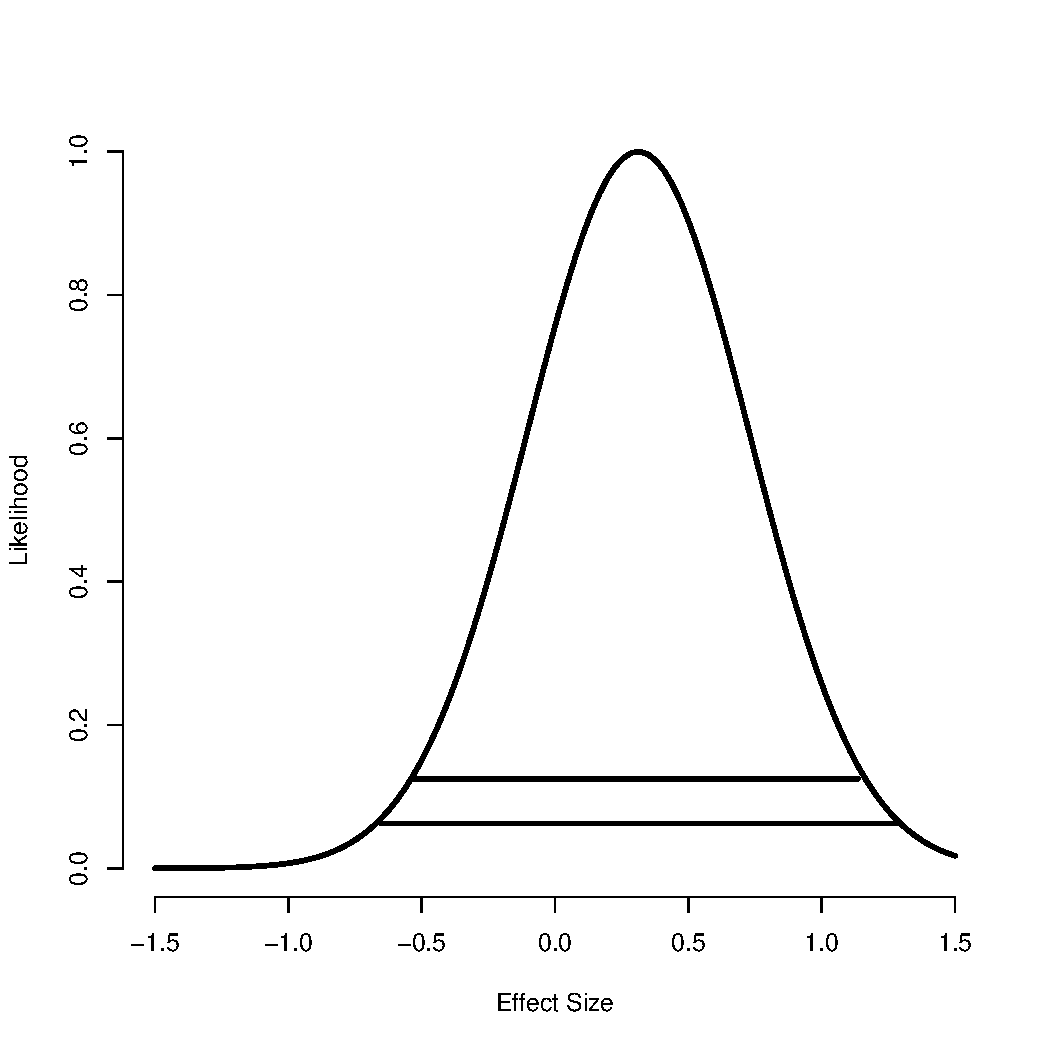
\includegraphics[scale=.3]{Lecture10ESlikelihood.pdf}
\end{center}
\end{frame}


\section{Unequal variances}
\begin{frame}\frametitle{Unequal variances}
  \begin{itemize}
  \item Note that under unequal variances
    $$
    \bar Y - \bar X \sim N\left(\mu_y - \mu_x, \frac{\sigma_x^2}{n_x} + \frac{\sigma_y^2}{n_y}\right)
    $$
  \item The statistic 
    $$
    \frac{\bar Y - \bar X - (\mu_y - \mu_x)}{\left(\frac{\sigma_x^2}{n_x} + \frac{\sigma_y^2}{n_y}\right)^{1/2}}
    $$
    approximately follows Gosset's $t$ distribution with degrees of freedom equal to
    $$
    \frac{\left(S_x^2 / n_x + S_y^2/n_y\right)^2}
    {\left(\frac{S_x^2}{n_x}\right)^2 / (n_x - 1) +
      \left(\frac{S_y^2}{n_y}\right)^2 / (n_y - 1)}
    $$
  \end{itemize}
\end{frame}


\begin{frame}\frametitle{Example}
\begin{itemize}
\item Comparing SBP for 8 oral contraceptive users versus 21 controls
\item $\bar X_{OC} = 132.86$ mmHg with $s_{OC} = 15.34$ mmHg
\item $\bar X_{C} = 127.44$ mmHg with $s_{C} = 18.23$ mmHg
\item $df=15.04$, $t_{15.04, .975} = 2.13$
\item Interval
$$
132.86 - 127.44 \pm 2.13 \left(\frac{15.34^2}{8} + \frac{18.23^2}{21} \right)^{1/2}
= [-8.91, 19.75]
$$
\end{itemize}
\end{frame}

\end{document}

